\chapter{Reservoir computing in out-of-plane artificial spin ice}\label{ch:Applications}
% TODO END: go through this chapter (and the others, probably) at the end and see if any comments with additional information can be put or merged anywhere.
\glijbaantje{If you find that you're spending almost all your time on theory,\\ start turning some attention to practical things; it will improve your theories.\\ If you find that you're spending almost all your time on practice,\\ start turning some attention to theoretical things; it will improve your practice.}{Donald Knuth}

\begin{adjustwidth}{2em}{2em} % TODO END: update once published.
	\begin{center}
		\textbf{Material from this chapter has also been published in:} \\
	\end{center}
	\vspace{1em}
	\begin{adjustwidth}{0em}{1.5em}
		\begin{itemize}
			\item[\cite{KUR-24}] A.~Kurenkov, J.~Maes, A.~Pac, G.~M.~Macauley, B.~Van~Waeyenberge, A.~Hrabec, and L.~J.~Heyderman.
			\newblock Perpendicular-anisotropy artificial spin ice with spontaneous ordering: a platform for neuromorphic computing with flexible timescales.
			\newblock \emph{ArXiV}, arXiv:\penalty0 2408.12182, 2024.
		\end{itemize}
	\end{adjustwidth}
	\vspace{.5em}
	\begin{center}
		\centering\rule{0.7\linewidth}{0.4pt}
	\end{center}
	\vspace{1em}
\end{adjustwidth}

The main factor that attracted attention towards OOP ASI for RC, was that they allow very efficient and relatively simple input and read-out methods to be used.
Early on in the \spinengine project, methods to read the state of OOP ASI had already been demonstrated experimentally on a small scale by ETHZ/PSI.
However, their potential for RC had not yet been investigated.
As \hotspice is well-suited for the simulation of OOP ASI, this presented an appropriate use-case for the software developed in~\cref{ch:Hotspice}. \par % Furthermore, the other simulator developed by the consortium (flatspin) only supports in-plane magnetisation. Furthermore, \hotspice is more accurate for OOP ASI than IP ASI due to the high degree of symmetry in the former.
Therefore, in this chapter, \hotspice will be used to assess the viability and characteristics of a couple of methods to achieve RC in OOP ASI.
It will be shown that RC is indeed possible in such systems by using an appropriate input and readout protocol.
This chapter starts with a discussion of the basic properties of OOP ASI and the motivation for researching them.
Then, the chapter is divided into two main parts, discussing thermally active and non-volatile ASI. % At first, the fabricated OOP ASI were not thermally active, though ASI which spontaneously relaxed to a checkerboard state was achieved later.
\section{Characteristics of OOP ASI}
\subsection{Structure of OOP nanomagnets} % Co/Pt multilayer, energy contributions
\label{sec:3:OOP_nanomagnet_PMA}
Where IP magnets mostly rely on shape anisotropy to create an easy axis, OOP magnets can be realised using interfacial anisotropy between the ferromagnetic material and the substrate.
One example of this is found at the interface between \ce{Co} and \ce{Pt}, as was used in the experimental OOP ASI fabricated within the context of the \spinengine project.
This \idx{perpendicular magnetic anisotropy} (PMA) acts in the immediate vicinity of the interface, where the magnetisation then prefers to align perpendicular to said interface. \par
Typically, a number of \ce{Co}-\ce{Pt} interfaces are stacked vertically, with the number and thickness of the ferromagnetic \ce{Co} layers then controlling the OOP anisotropy.
The ferromagnetic layers in such stacks are typically made to be very thin for two main reasons.
Firstly, since the PMA only acts at the interface, it does not increase for thicker layers.
Secondly, recall that the energy associated with \xref{shape anisotropy} increases with volume ($\EB=K_\mathrm{u}V$), so a maximal number of layers for a given amount of ferromagnetic material is preferable for PMA to counteract the in-plane shape anisotropy.
We will elaborate on the interplay between these energy contributions later in~\cref{sec:3:E_contributions}. \par
Other factors contribute to the anisotropy as well, e.g. a non-linear dependence on the \ce{Pt} layer thickness due to the RKKY interaction~\cite{RKKY_RK,RKKY_K,RKKY_Y}.
However, this coupling is likely not dominant in a \ce{Co}-\ce{Pt} stack, as \ce{Pt} nearly satisfies the Stoner criterion~\cite{PtMagneticOrder}.
Since the \ce{Pt} is combined with a ferromagnetic material (\ce{Co}), it is thought that this induces a ferromagnetic coupling between \ce{Co} layers in spite of the RKKY interaction, at least for reasonable \ce{Pt} thicknesses up to a few \SI{}{\nano\metre}~\cite{PerpendicularMagnetizationASI}.

\subsection{ASI ground state} % TODO: make sure this paragraph still feels right, now that the non-volatile ASI is not the next section but is all the way at the end. Might have to move some sentences that do not make much sense for thermal ASI. But then again, this is still a general OOP ASI discussion, so we should probably keep it broad.
The ground state of any system used for RC is crucial, as it dictates which input methods will induce desirable dynamics in the system and which input protocols will be ineffective, particularly for a non-volatile system.
For most OOP spin ices, the ground state exhibits some form of antiferromagnetic (AFM) ordering due to the magnetostatic interaction, which always encourages opposite magnetisation between two neighbouring OOP magnets.
As is the case for any ASI, the ground state is at least twofold degenerate, because all interactions are symmetric under magnetisation reversal. \par
Depending on the particular lattice upon which the OOP magnets are placed, frustration may (e.g. triangle/Cairo; \crefSubFigRef{fig:2:ASIs}{j,l}) or may not (e.g. square/honeycomb; \crefSubFigRef{fig:2:ASIs}{i,k}) be present due to the local AFM ordering.
In the absence of frustration, the symmetry of the system imposes exactly two opposite ground states.
Conversely, if frustration is present, then not all local interactions can be satisfied simultaneously, making the global ground states of the system hard to reach. \par % Locally, vertices where magnets meet will have a degenerate ground state, giving rise to mobile domains dictated by frustration.
For the OOP square-lattice ASI (\crefSubFigRef{fig:2:ASIs}{i}) in particular, which we focus on in this chapter, the ground state adopts an AFM checkerboard pattern of `up' ($\uparrow$) and `down' ($\downarrow$) magnetisation.
We focus on the square-lattice system because it is the simplest example of a non-frustrated OOP ASI.
The results obtained for this system will be applicable to most other non-frustrated OOP ASI because they all exhibit a twofold degenerate AFM ground state.
Non-frustrated lattices with the same NN spacing can only differ in their magnetostatic interactions for next-nearest neighbours and beyond.
However, since this interaction decays rapidly with distance, the ground state is typically dictated by the NN, which prefer anti-parallel alignment.
Therefore, if every closed NN loop in an OOP lattice contains an even number of magnets, as is the case for the square and honeycomb lattices, then the lattice is unlikely to exhibit geometric frustration.

\subsection{Input and readout: experiment to simulation}
While it is possible to use an external field to switch both IP and OOP nanomagnets, this is undesirable in a real device due to stray fields and the need for bulky magnets.
The main allure of OOP ASI for RC stems from the existence of efficient input and readout mechanisms for such OOP magnets.
Input can be applied via spin-orbit torque (SOT)~\cite{SOT_FM_AFM,SOTswitchingCoPt}, while the system can be read out using the anomalous Hall effect (AHE)~\cite{AHE}.
Both of these only require a current to be passed through an underlayer that is electrically connected to the sample, and were explained earlier in the introduction (\cref{sec:1:ASI_IO}).
% Nonetheless, external fields are often used for input anyway in the lab during the first stages of development, because they are easier to handle than the more complicated methods that would be used in a real device. By the end of the project, Alex had used SOT in his actual devices.

\paragraph{Input by spin-orbit torque}
In the experimental system, the intent was to apply input data by using SOT~\cite{SOTswitchingCoPt} to switch the OOP magnets.
Compared to an \xref{external magnetic field}, this allows far greater control over the stimulus applied for each input bit, and can more easily be integrated on-chip without generating significant stray fields. \par
Since the model used by \hotspice does not use torques, but is rather based on switching energies, SOT can not directly be modelled as a torque in our simulations.
However, the net desired effect of SOT in our application is deterministic switching of magnets, which can be achieved if in-plane symmetry breaking is present in the system~\cite{SOT_Roadmap}. % SOT_Roadmap mentions symmetry breaking several times, very useful resource
Such broken symmetry combined with SOT can be used to create a preferential magnetisation direction, which can be modelled in \hotspice as an additional external field $B_z$.
This is a crude approximation to fit SOT into the Ising-like model; the modelled field $B_z$ is not necessarily related to the field-like SOT torque~\cite{SOT_firstprinciplesCoPt}, though a non-linear relationship between the SOT current density and the modelled field $B_z$ will exist.
The exact form of this relationship is currently irrelevant for our RC purposes, because it only constitutes an additional non-linear transformation on the input which does not fundamentally change the RC performance of the OOP ASI itself.
% In the case without symmetry breaking, the effect may be modelled as a temporary reduction of the PMA, as in reality a sufficiently strong SOT (applied over multiple $\tau_0$) will push the magnetic moment in-plane~\cite{SOT_Roadmap}, after which it falls back randomly (with higher likelihood to the lowest energy state, I suppose). But this approach raises multiple additional questions: is it meaningful to reduce the barrier only slightly?

\paragraph{Readout by anomalous Hall effect}
In our paper~\cite{KUR-24}, \textit{A. Kurenkov} experimentally demonstrated electrical readout of the average magnetisation $\llangle s \rrangle$ using the anomalous Hall effect~\cite{AHE}.
This can therefore be used as a magnetic state readout in the simulations.
However, reservoir computing benefits from having multiple readout values, so we will use the average magnetisation of each lattice column $i$ to populate our readout vector $y_i(t)$. \par % Fig. 6a in paper
A discussion about the experimental feasibility of such a grid of local readouts is given in Supplementary Information 7 of our paper~\cite{KUR-24}.
In short, by adding more electrodes to the Hall bar --- the conductive layer underneath the ASI used to measure the magnetic state through the AHE --- inhomogeneities in the current density distribution result in different currents flowing through the various nanomagnets.
This consequently results in unequal contributions to the Hall resistance, providing a way to differentiate between magnets.
Individual states of the nanomagnets, not just $\llangle s \rrangle$, can be extracted through a set of linear operations.
In the context of reservoir computing, this means that such a readout approach with multiple electrodes can be computationally equivalent to knowing the exact magnetic configuration of the system.

%We will later notice that simple stimuli are not sufficient for RC in this (non-volatile) system, and instead more complicated patterns will have to be used to meaningfully address the system. However, the practical implementation of such complicated stimuli requires more complicated current line layouts, which also cannot interfere with the readout. This proves to be a conundrum, which I will address later again.

\section{Thermally active OOP ASI}
\subsection{Energy contributions} \label{sec:3:E_contributions}
Thermally active OOP ASI are hard to manufacture, because they must strike a delicate balance between several strong energy contributions to end up in an OOP state with a net energy barrier of only several tens of $\kBT$ at most.
To appreciate this difficulty, let us first take a closer look at the various energy contributions in the system --- ranging from local anisotropy to large-scale interactions --- and their dependence on the geometrical structure of the OOP magnets.
\begin{enumerate}
	\item \textbf{Perpendicular magnetic anisotropy} constitutes the largest contribution to the total OOP anisotropy.
	Its interfacial origin and characteristics have been discussed earlier in this chapter (see \cref{sec:3:OOP_nanomagnet_PMA}). % Anisot E: \approx\SI{1.1e-16}{\joule}
	\item \textbf{Shape anisotropy}\indexlabel[nolabel]{shape anisotropy} of each layer due to their \xlabel[nolabel]{demagnetising field}.
	It is of a similar order of magnitude as the PMA, but of opposite sign, favouring an IP magnetisation rather than OOP.
	This contribution was also discussed earlier, see~\cref{sec:2:shape_anisotropy}~and~\ref{sec:3:OOP_nanomagnet_PMA}. % Demag E: \approx\SI{-1.6e-16}{\joule}
	\item \textbf{Inter-layer magnetostatic interaction}.
	The separate FM layers within a single stack also interact, as they can all be considered as separate vertically stacked magnets.
	This vertical stacking provides an additional contribution to the OOP anisotropy because, in general, the magnetisation of separate magnets prefers to point along the axis connecting those magnets.
	One can think of this effect as being similar to the shape anisotropy, but on the scale of separate layers rather than individual atomic magnetic moments.
	This contribution aids the PMA in stabilising the OOP anisotropy, counteracting the \xref{demagnetising field}, but is smaller in magnitude. % Cross MS E: \approx\SI{0.5e-16}{\joule}
	\item \textbf{Inter-magnet magnetostatic interaction} is the only contribution --- besides external input --- that distinguishes between the $\uparrow$ and $\downarrow$ magnetisation states.
	All aforementioned energy contributions are internal to individual OOP magnets, making the \xref{magnetostatic interaction} the sole reason for the AFM ground state of the OOP ASI. % E_MS: \lesssim\SI{1.1e-17}{\joule}
	\item \textbf{Input}.
	In simulations, an \xref{external magnetic field} is used as a proxy to model SOT.
\end{enumerate}
For a system to exhibit spontaneous switching, the first three of these contributions should mostly cancel out --- to the level where their combined influence is of the same order of magnitude as the inter-magnet magnetostatic interaction, which is usually at least an order of magnitude weaker than the other contributions separately.
As we will see in~\cref{sec:3:relaxation}, achieving spontaneous thermal ordering to the ground state may require even finer control.

\paragraph{Magnet geometry}
\label{sec:3:OOP_geometry}
% The geometry of nanomagnets in an OOP ASI is shown schematically in~\cref{fig:3:OOP_geometry}.
% TODO: make own figure of nanomagnets?

The magnets considered here are round with a diameter $D_\mathrm{NM}$ and consist of $N_{\ce{Co}}$ layers of \ce{Co} with a thickness $t_{\ce{Co}}$, separated and surrounded by \ce{Pt} layers of thickness $t_{\ce{Pt}}$.
They are placed in an ASI where the lateral spacing between magnets is $S_\mathrm{ASI}$ --- resulting in a lattice parameter $a=D_\mathrm{NM}+S_\mathrm{ASI}$ in a square lattice. \par
These five geometrical parameters have a profound effect on the balance between the aforementioned energy contributions, as summarised in~\cref{tab:3:interactions_geometry}.
The polynomial dependence of some of these relations makes the system quite hard to control: a slight manufacturing difference can yield a vastly different net OOP anisotropy, possibly inhibiting the spontaneous formation of a checkerboard ground state.
Note that the magnetostatic interactions depend on the square of the ferromagnetic volume $V=n_{\ce{Co}} t_{\ce{Co}} D_\mathrm{NM}^2$.

\xtable[tab:3:interactions_geometry]{
	Dependence of the energy components present in OOP ASI on the geometrical parameters.
	$x$ represents the parameter at the top of the column.
	The magnet centre-to-centre distance $r = D_\mathrm{NM} + S_\mathrm{ASI}$.
	PMA depends non-trivially on $t_{\ce{Pt}}$.
	Empty cells indicate no significant dependence.
}{
	\begin{tabular}{r|c|c|c|c|c}
		\multicolumn{1}{r}{} & \multicolumn{1}{c}{$t_{\ce{Co}}$} & \multicolumn{1}{c}{$n_{\ce{Co}}$} & \multicolumn{1}{c}{$D_\mathrm{NM}$} & \multicolumn{1}{c}{$t_{\ce{Pt}}$} & \multicolumn{1}{c}{$S_\mathrm{ASI}$} \\
		\hline \hline
		PMA (interfacial anisotropy) &  & $x$ & $x^2$ & $\aquarius$ &  \\
		\hline
		Shape anisotropy (demag) & $x^2$ & $x$ & $x^4$ &  &  \\
		\hline
		Inter-layer MS interaction & $x^2$ & $x^2$ & $x^4$ & $x^{(< -3)}$ &  \\
		\hline
		Inter-magnet MS interaction & $x^2$ & $x^2$ & $x^4$ &  & $r^{(< -3)}$ \\ % S_ASI: $>r^{-3} + \frac{3}{16}D_\mathrm{NM}^2 r^{-5} $
		\hline
		Input (external field) & $x$ & $x$ & $x^2$ &  &  \\
		\hline
	\end{tabular}
}

These five geometrical parameters are bounded by several physical and practical constraints.
Note that the numerical values of the limits given below are only indicative and may depend on the exact values of the other geometrical parameters.
\begin{itemize}
	\item \textbf{FM layer thickness} $\boldsymbol{t_{\ce{Co}}} \lesssim \SI{1.45}{\nano\metre}$. \newline
	This upper bound was experimentally determined~\cite{KUR-24} and is imposed by shape anisotropy.
	Layers must be sufficiently thin to maintain OOP anisotropy, as \xref{shape anisotropy} is proportional to volume (and hence $\propto t_{\ce{Co}}$) while the PMA is mostly independent of $t_{\ce{Co}}$. \par % t_{\ce{Co}} controls the demag compensation of $K_u$.
	The closer the thickness is to this upper bound, the lower the effective OOP anisotropy will be.
	Therefore, non-volatile ASI must steer clear of this limit, while thermally active ASI generally try to approach this limit as close as possible.
	As such, this geometrical parameter is often key for balancing the energy landscape.
	\item \textbf{Separation between magnets} $\boldsymbol{S_\mathrm{ASI}} \gtrsim \SI{20}{\nano\metre}$. \newline
	This constraint is of a practical nature, as the minimal size of lateral geometrical features is limited by the accuracy of the lithographic process. \par
	The separation only affects the strength of the magnetostatic interaction between neighbouring magnets, as approximated in \hotspice by \cref{eq:2:E_MS} and the second-order correction of \cref{eq:2:E_MS_order2}.
	In ASI, a strong MS coupling --- hence low $S_\mathrm{ASI}$ --- is often preferred.
	However, for thermally active ASI we will soon see that excessively strong MS coupling is detrimental, resulting in a ``sweet spot'' of MS coupling energies.
	\item \textbf{Number of layers} $\boldsymbol{n_{\ce{Co}}} \lesssim 8$. \newline
	This limit is of a practical nature as well --- property drift during deposition of successive layers makes it harder to achieve small $S_\mathrm{ASI}$ for increasingly tall stacks. \par
	Note that the number of layers does not affect the balance between PMA and shape anisotropy, as the number of interfaces per amount of magnetic material remains constant.
	However, since MS interactions grow $\propto n_{\ce{Co}}^2$, the inter-layer coupling --- and with it the net OOP anisotropy --- becomes increasingly significant for a large number of layers.
	\item \textbf{Diameter} $\boldsymbol{D_\mathrm{NM}} \lesssim \SI{200}{\nano\metre}$. \newline
	Magnets wider than this limit were observed to take on multi-domain states~\cite{KUR-24}, as their demagnetisation energy becomes dominant due to its rapid $\propto D_\mathrm{NM}^4$ growth.
	Even though in-plane magnets without uniform magnetisation have been used for computation~\cite{gartside2022reconfigurable}, we did not intend to use this in the OOP systems.
	Furthermore, the \hotspice simulator requires a single-domain magnetisation state for its Ising-like model to be applicable. \par
	The diameter can be used to control the relative strength between PMA and shape anisotropy and greatly affects the inter-magnet MS coupling.
	\item \textbf{Spacer layer thickness} $\boldsymbol{t_{\ce{Pt}}} \gtrsim \SI{0.4}{\nano\metre}$. \newline
	Thinner layers may become discontinuous, which is detrimental to the PMA.
	On the other hand, a thin spacer layer maximises the net OOP anisotropy due to the $\approx t_{\ce{Pt}}^{-3}$ inter-layer MS coupling dependence.
	Note that $t_{\ce{Pt}}$ must still be chosen appropriately to promote FM coupling between layers while maintaining the interfacial anisotropy. % Accounting for various effects such as RKKY coupling
\end{itemize}

In the particular case of the thermally active OOP ASI fabricated within the \spinengine project, the nanomagnets consist of $n_{\ce{Co}}=7$ ferromagnetic layers of $D_\mathrm{NM}=\SI{170}{\nano\metre}$ diameter and $t_{\ce{Co}} \approx \SI{1.45}{\nano\metre}$ thickness, with $t_{\ce{Pt}} \approx \SI{0.8}{\nano\metre}$ spacing layers in between.
The edge-to-edge spacing between neighbouring magnets is $S_\mathrm{ASI}=\SI{30}{\nano\metre}$, unless specified otherwise.
The saturation magnetisation $M_\mathrm{sat}$ is thickness-dependent~\cite{CoFilmPropertiesCVD}, with a value of $M_\mathrm{sat}=\SI{1063}{\kilo\ampere\per\metre}$ reported for thicknesses in the \SI{}{\nano\metre} range~\cite{Msat_Co}.

\subsection{Relaxation characteristics}
\label{sec:3:relaxation}
To better inform our choices for RC in thermally active ASI, it is essential to familiarise ourselves with its spontaneous relaxation process.
In this section, we numerically investigate this process with \hotspice by initialising an OOP ASI in a uniform ($\uparrow$) state and subsequently observing its decay towards the checkerboard ground state over a certain timespan.
In the Ising-like model used by \hotspice, two essential system parameters remain, denoted as
\begin{itemize}[leftmargin=4.1em]
	\item[$\boldsymbol{\EEA}$ ---] the energy barrier of a single non-interacting OOP magnet due to the net OOP anisotropy.
	This is the combined contribution of PMA, shape anisotropy and the inter-layer magnetostatic interaction.
	\item[$\boldsymbol{\EMC}$ ---] the magnetostatic coupling energy between nearest neighbours.
	This is responsible for the relaxation to the ground state.
\end{itemize}
Due to the N\'eel-Arrhenius switching law~\eqref{eq:2:Néel}, it is more appropriate to write dimensionless energies ($\EEA/\kBT$ and $\EMC/\kBT$), as it is only this ratio --- not the absolute value of the energies or temperature --- that controls the switching times. \par
In real ASI, manufacturing inevitably introduces imperfections.
Slight geometrical variations can result in a significant variance of the net OOP anisotropy between magnets~\cite{Budrikis2012,DisorderGroundStateASI}.
In simulations, this will be modelled by sampling $\EEA$ from a normal distribution: unless otherwise specified, a standard deviation $\sigma(\EEA) = \SI{5}{\percent}$ is used~\cite{Farhan2013}.
This provides pinning sites for domain walls, making the relaxation process more reproducible: such ``consistent variation'' within an ASI could ultimately be beneficial for RC by providing a richer output space. \par
The effective energy barrier $\EBeff$ of a magnet $i$ can then symbolically be written as
\begin{equation}
	\label{eq:3:OOP_relaxation_EBeff}
	\EBeff{}_{,i}(t) = \EEA \Big(1 + \sigma\ab(\EEA) \sampi_i \Big) + \EMC \sum_j s_i(t) D_{ij} s_j(t)
\end{equation}
with $\sampi$ a random value from a standard normal distribution and $D_{ij}$ a factor proportional to the magnetostatic interaction energy between magnets $i$ and $j$. \\\par

The relaxation process can be tracked by the normalised average magnetisation $\mavg = \abs{\llangle s \rrangle}$ and the local antiferromagnetic parameter $\qNN = (1 - \langle s_i s_{i+1} \rangle)/2$.
In the uniform state --- where all magnetic moments point `up' --- their values are $\mavg=1$ and $\qNN=0$.
During relaxation, they transition to $\mavg=0$ and $\qNN=1$, corresponding to a checkerboard ground state.
Note that, while for a random state $\qNN \approx 0.5$, a value of $\qNN=0.5$ does not necessarily imply a random state. \par

\cref{fig:3:OOP_relaxation} shows relaxation profiles for a few combinations of $\EEA$ and $\EMC$, providing some insight into the relaxation process.
Each panel shows the mean, standard deviation and 1st/99th percentile of $\mavg$ and $\qNN$ over 200 relaxations --- this variance is both due to the randomness of N\'eel-Arrhenius switching and because each relaxation used unique randomly sampled $\EEA$ for individual magnets, in accordance with the $\sigma(\EEA) = \SI{5}{\percent}$ variation.
Each relaxation consisted of at most $40N$ switches using the first-switch method, as this is sufficient for the system to achieve equilibrium.
The size of the ASI does not significantly affect the relaxation process, apart from reducing the spread on these traces.

\xfig{3_RC_OOP/OOP_relaxation.pdf}{
	\label{fig:3:OOP_relaxation}
	Dependence of the ordering timescale on the energy balance between net OOP anisotropy $\EEA$ and nearest-neighbour magnetostatic coupling $\EMC$ in an $11 \times 11$ OOP square-lattice ASI. % This system size was chosen because it matched the size of our fabricated systems discussed later.
	The ASI is initialised in a uniform magnetic state with all spins pointing `up' and is released at $t = 0$, after which the lattice relaxes to lower energies.
	Blue traces show the absolute value of the normalised average magnetisation $\mavg$ while orange traces represent the local antiferromagnetic parameter $\qNN$.
	Each trace shows the mean (central line), standard deviation (central shaded area), and 1st/99th percentile (outer shaded area) of 200 repeated relaxations with randomly sampled $\EEA$ profiles.
	At most $40N$ switches are simulated for each relaxation.
	The green shaded region highlights stage~$\circled{2}$ of ordering.
	The simulations are either stopped after \SI{e4}{\second} or $40N$ switches --- whichever is reached first.
	\textbf{The insets} show the resulting final magnetic states, where white (black) indicates up (down) spins.
}

\subsubsection{Logarithmic relaxation}
Most strikingly, by using a logarithmic scale for the time axis, both $\mavg$ and (to a lesser extent) $\qNN$ trace a very straight line during relaxation.
Because of this \idx{logarithmic relaxation}, the first switches occur on a vastly different timescale than the last --- each subsequent switch occurs on average $x$ times later than the previous switch ($t_{i+1} = x t_i \Rightarrow t_n = t_0 x^n$). \par
The cause of this is the magnetostatic interaction\footnote{
	Without the \xref{magnetostatic interaction}, the system would simply be a non-interacting ensemble of nanomagnets, which is known to relax to the ground state exponentially.
	This is the opposite of logarithmic relaxation; quantities like $\mavg$ would only show up as straight lines when using a linear time axis and logarithmic y-axis.
	% Exponential decay would be much easier to work with for temporal input, but having no MS coupling defeats the point of using an ASI for some nonlinearity.
}.
Initially, all magnets are in a high-energy state as they all point in the same direction.
After a certain amount of time, a first magnet will switch, thereby slightly stabilising all other magnets in the ASI to some degree according to the second term of~\cref{eq:3:OOP_relaxation_EBeff}.
Whichever magnet randomly switches next will therefore experience a slightly higher effective energy barrier $\EBeff$ than before.
On average, this means that the effective barrier $\max(\EBeff)$ of the most unstable magnets in the system --- those most eager to switch next --- will increase linearly with the amount of switched magnets.
The N\'eel-Arrhenius equation~\eqref{eq:2:Néel} translates this to an exponentially increasing switching time. \\\par

\cref{fig:3:OOP_relaxation} also shows that the slope generally becomes less steep for higher coupling $\EMC$.
Following the previous discussion, we now understand that high coupling results in a greater decrease of $\EBeff$ per switch, and consequently a larger exponential increase in the switching time.
Meanwhile, the net OOP anisotropy $\EEA$ only affects the timescale of the relaxation --- it does not affect the slope, but simply shifts the relaxation curves along the (logarithmic) time axis.
Therefore, to achieve an ASI that exhibits a particular relaxation timescale, accurate control of $\EEA$ on a scale of $\sim 10\kBT$ is required. \par
The effects of $\EMC$ and $\EEA$ can be quantified by fitting a logarithmic curve to the mean relaxation curves of the nine panels in ~\cref{fig:3:OOP_relaxation}, yielding the general trends
\begin{equation}
	\label{eq:3:relaxation_fit_ab}
	\mavg = a \log_{10}(t \nu_0) + b \quad \mathrm{with} \quad \begin{cases}
		a \approx -\frac{\kBT}{2\EMC} \, \mathrm{,} \\
		b \approx \frac{\kBT}{6\EMC}(\frac{\EEA}{\kBT} - 1.5) - 0.05 \, \mathrm{.}
	\end{cases}
\end{equation} % TODO: more rigorous fit?

% Note that the change in slope $a$ and the offset $b$ compensate to some extent such that the final switches ($\mavg \rightarrow 0$) occur around the same time nearly independently of $\EMC$.
% The intercept of the fit for $\mavg=0$ is indeed far less sensitive to $\EMC$ than to $\EEA$:
% \begin{equation}
%  	t_{\mavg=0} = \frac{10^{-b/a}}{\nu_0} = \frac{10^{\frac{\EEA - 0.3 \EMC}{3\kBT} - 0.5}}{\nu_0} \mathrm{.}
% \end{equation}

\subsubsection{Two-stage relaxation}
While $\mavg$ follows a near-perfect logarithmic relaxation, $\mavg \approx 0$ is reached earlier than the perfect checkerboard ordering $\qNN = 1$ --- most strikingly in panels 6 and 9 of~\cref{fig:3:OOP_relaxation}.
This is accompanied by a decreased ordering rate $\frac{\partial \qNN}{\partial \log(t)}$, marking the transition between stage~$\circled{1}$ and~$\circled{2}$ of relaxation.
The latter is indicated by the green shaded area in the figure. \par
This can be understood by considering the microstate of the ASI: to this end, the final state of each panel in~\cref{fig:3:OOP_relaxation} is shown as an inset.
Panels 1 and 2 show the system during the logarithmic relaxation of both $\mavg$ and $\qNN$ in stage~$\circled{1}$.
Here, many magnets still have three or four NN with the same magnetisation state, causing random magnets to switch and small checkerboard domains to nucleate throughout the system.
Because these domains are twofold degenerate, the perfect checkerboard ordering is not reached directly.
Instead, expanding domains are likely to be separated by domain walls, as seen in panels 3 and 4 which have just barely reached stage~$\circled{2}$.
From this point on, a further increase in $\qNN$ can only\footnote{
	If the magnetostatic coupling $\EMC$ is insufficient, a perfect checkerboard ordering will not be achieved and $\qNN$ may not increase much further --- in panel 7 of~\cref{fig:3:OOP_relaxation}, $\qNN$ settles around $\approx 0.8$.
} be achieved by switching magnets that are part of a domain wall.
However, even though domain wall magnets are the least stable magnets in the system, they still typically have 3 stabilising NN, resulting in a significant effective energy barrier that depends on both $\EEA$ and $\EMC$.
Furthermore, when a domain wall magnet finally switches, it simply moves the domain wall by one lattice unit without significantly altering the macrostate of the system.
This is in stark contrast with stage~$\circled{1}$, where the macrostate was constantly changing.
Only when the domain wall randomly encounters a domain wall of opposite polarity or an edge of the system, can the total length of domain walls in the system decrease --- as occurs between panels 5 and 8.
This process is more akin to a random walk, and therefore has a polynomial time dependency rather than a logarithmic one.
For this reason, stage~$\circled{2}$ shows up in~\cref{fig:3:OOP_relaxation} as a sudden increase of $\qNN$ after a plateau, as most clearly seen in panel 9. \par
Once the system has finally approached the checkerboard state with $\mavg \rightarrow 0$ and $\qNN \rightarrow 1$, random thermal fluctuations will still cause small excursions to $\mavg > 0$ and $\qNN < 1$.
These are generally more pronounced for low coupling $\EMC$, as can clearly be seen in the $\EEA = 20\kBT$ row of~\cref{fig:3:OOP_relaxation}.
This is because $\EMC$ is the only factor responsible for order in the system: low coupling makes magnets less inclined to reside in the ground state, giving the opportunity for multiple magnets to be in an unstable state at once and drive $\mavg$ further from 0.

%\paragraph{Miscellaneous remarks}
%During the relaxation process, one may be inclined to draw the conclusion from~\cref{fig:3:OOP_relaxation} that larger $\EMC$ yields more random variation.
%This is mostly an illusion due to the steep slope of the relaxation for low $\EMC$: while the lower slope for $\mavg$ increases the random variation along the temporal axis, the vertical spread actually decreases for larger $\EMC$. \par

\subsubsection{Phase diagram}
A stronger coupling $\EMC$ causes faster decay of $\mavg \rightarrow 0$: in panels 4--6 of~\cref{fig:3:OOP_relaxation}, the time to reach $\mavg \sim 0$ decreases from $\approx \SIrange{e3}{10}{\second}$.
However, strong coupling does not necessarily result in faster ordering $\qNN \rightarrow 1$ --- as panels 8 and 9 clearly illustrate --- because domain wall magnets typically have 3 oppositely magnetised nearest neighbours, resulting in a net stabilising effect proportional to $\EMC$ (and $\EEA$).
Therefore, for a system to reach the checkerboard state on a given timescale, a sufficiently low $\EMC$ and $\EEA$ are required. \par
This is most clearly seen in phase diagrams like~\cref{fig:3:OOP_relaxation_continuous}, which summarise the values of $\mavg$ and $\qNN$ at $t = \SI{e4}{\second}$ (i.e., the maximum time in \cref{fig:3:OOP_relaxation}) over a wide range of $\EEA$ and $\EMC$.
This encompasses the nine $(\EMC,\EEA)$ combinations of the various panels in~\cref{fig:3:OOP_relaxation}, as indicated by grey numbered crosses in~\cref{fig:3:OOP_relaxation_continuous}. \par
Five distinct regions can be distinguished.
In region~$\mathrm{I}$ (panel 1), weak coupling and high anisotropy result in a non-volatile system --- as used in the previous section --- where no spontaneous switches occur and $\mavg = 1$ and $\qNN = 0$ remain unchanged.
Increasing the $\EMC/\EEA$ ratio shifts the system though the transient region~$\mathrm{II}$ (panel 2), characterised by decreasing $\mavg$ and increased ordering.
Further increase of $\EMC/\EEA$ shifts the system to region~$\mathrm{III}$ (panel 6) with $\mavg \approx 0$ but $\qNN \neq 1$, characteristic of stage~$\circled{2}$.
Any further increase of $\EMC/\EEA$ does not affect the average magnetisation or ordering at $t = \SI{e4}{\second}$ --- unless both $\EEA$ and $\EMC$ are sufficiently small, as in regions~$\mathrm{IV}$ and~$\mathrm{V}$. \par
Region~$\mathrm{IV}$ (panel~9) is the only region where the system spontaneously achieves the checkerboard ground state.
In~\cref{fig:3:OOP_relaxation_continuous}, it is delineated by the dotted black line that envelops a region with $\qNN \geq 0.95$.
Reducing $\EMC$ too much puts the system in region~$\mathrm{V}$ (panel 7), where the system is superparamagnetic at this timescale.
For $t = \SI{e4}{\second}$, region~$\mathrm{V}$ extends upwards to $\EEA \lesssim 32 \kBT$, since the N\'eel-Arrhenius switching law states that nanomagnets with such anisotropy have a mean switching time $\lesssim \exp(32)/\nu_0 \approx \SI{e4}{\second}$.
The main region of interest --- region~$\mathrm{IV}$ with $\qNN \approx 1$ --- is therefore constrained from the left by the superparamagnetic regime, from the top by the transient/frozen regime, and from the right by states in which domain boundaries are too stable at the given timescale. \par

\xfig{3_RC_OOP/OOP_relaxation_continuous.pdf}{
	\label{fig:3:OOP_relaxation_continuous}
	Phase diagrams of the normalised average magnetisation $\mavg$ and the local antiferromagnetic parameter $\qNN$ as a function of net out-of-plane anisotropy $\EEA$ and nearest-neighbour magnetostatic coupling $\EMC$ at $t=\SI{e4}{\second}$.
	Five regions can be distinguished: $\mathrm{I}$ -- frozen state, $\mathrm{II}$ -- transient states, $\mathrm{III}$ -- state with domains and domain boundaries, $\mathrm{IV}$ -- checkerboard ordering, $\mathrm{V}$ -- superparamagnetic state.
	The white and black dotted line respectively correspond to $\mavg = 0.05$ and $\qNN = 0.95$.
	The nine panels of~\cref{fig:3:OOP_relaxation} are indicated by grey crosses.
	The three symbols correspond to the experimental lattices shown in~\cref{fig:3:MFM_grid} with nanomagnet diameter $D_\mathrm{NM} = \SI{170}{\nano\metre}$, \ce{Co} thickness $t_{\ce{Co}} = \SI{1.45}{\nano\metre}$ and nanomagnet separations $S_\mathrm{ASI} = \SI{20}{\nano\metre}$ (circle), $S_\mathrm{ASI} = \SI{25}{\nano\metre}$ (triangle), $S_\mathrm{ASI} = \SI{30}{\nano\metre}$ (cross).
}

The phase diagrams in~\cref{fig:3:OOP_relaxation_continuous} are snapshots at $t = \SI{e4}{\second}$ and, with increasing time, region~$\mathrm{IV}$ will expand and the boundaries between the different regions will shift upwards.
Therefore, if the observation is long enough and $\EMC$ is non-negligible, a system located in the frozen region at $t = \SI{e4}{\second}$ may eventually find itself in the more ordered regions~$\mathrm{II}$, $\mathrm{III}$ or~$\mathrm{IV}$.
However, due the exponential character of the N\'eel-Arrhenius law, this shift will be minimal and region~$\mathrm{IV}$ will not become much bigger than in~\cref{fig:3:OOP_relaxation_continuous} for any realistic timescale~\cite{KUR-24}.

\subsubsection{Exchange-coupled system} % TODO: expand, could be omitted if not sufficiently worked out

\subsubsection{Summary}
The state of an OOP ASI is defined by the net OOP anisotropy $\EEA$, magnetostatic coupling $\EMC$ and elapsed time $t$.
Increasing $\EMC$ causes the relaxation to occur over a larger amount of timescales.
Meanwhile, $\EEA$ controls the timescale of the relaxation but does not affect the amount of timescales over which the relaxation occurs.
For reservoir computing purposes, a sufficiently low $\EEA$ and $\EMC$ are required --- but not too low, to maintain OOP anisotropy and a ground-state checkerboard ordering, respectively.
Therefore, practical applications exploiting systems with specific dynamics will require careful adjustment of the lattice and nanomagnet dimensions~\cite{KUR-24}.

\subsection{Fitting MFM images}\label{sec:3:MFM}
Based only on the magnet geometry --- determined by the various geometrical parameters discussed earlier in~\cref{sec:3:OOP_geometry} --- it is hard to predict the net OOP anisotropy $\EEA$ and magnetostatic coupling $\EMC$ of a manufactured ASI.
For typical nanomagnet dimensions (7 layers of $t_{\ce{Co}} \approx \SI{1.45}{\nano\metre}$ with $D_\mathrm{NM} \approx \SI{170}{\nano\metre}$), some of the aforementioned energy contributions are on the order of several $1000 \kBT$, as we discuss in more detail in~\ccite{KUR-24} (Supp. 4). % --- especially PMA and shape anisotropy, which have opposite sign and therefore mostly cancel out.
Due to manufacturing defects, the discrepancy between theoretical estimates of these energy contributions and their real magnitudes can easily exceed $100 \kBT$. % Theoretically, $\EEA$ of an isolated magnet (as manufactured by Alex and observed to be part of a thermally relaxing OOP ASI) is $\approx\SI{-3.6e-18}{\joule} = \SI{-22.5}{\electronvolt} = -871\kBT$ which is far too large to get thermal switching. Furthermore, it is negative, implying an IP magnetisation. This discrepancy between Mathematica and reality could be due to non-coherent reversal, lowering the real energy barrier.
However, we just saw that $\EEA$ and $\EMC$ must not exceed several tens of $\kBT$ if a system is to spontaneously reach the checkerboard ground state.
It is therefore inappropriate to calculate $\EEA$ and $\EMC$ theoretically --- they must be empirically determined from manufactured ASI. \\\par
For this reason, \textit{A. Kurenkov} manufactured several $11 \times 11$ OOP square-lattice ASI, initialised them in the `up' state by a \SI{0.9}{\tesla} OOP field and measured their state using MFM at different time intervals since initialisation.
For each of these MFM images, the values of $\mavg$ and $\qNN$ can be determined.
The knowledge of these quantities at different moments in time can then be used to fit this data to simulated relaxations, like the ones in~\cref{fig:3:OOP_relaxation}, by varying simulation parameters like $\EEA$ and $\EMC$.

\subsubsection{Bayesian optimisation}
Any fitting procedure requires an appropriate metric $\eta$ to determine the quality of the fit.
For this, we will use the random distribution of both $\mavg$ and $\qNN$ at the times of measurement $t_i$, as previously seen in~\cref{fig:3:OOP_relaxation}.
These distributions are each characterised by a mean and standard deviation, which can be determined from repeated simulations --- typically, 200 relaxations are used. % We embrace the Monte Carlo nature of \hotspice.
Therefore, each experimental data-point lies some amount of standard deviations away from the mean of this simulated distribution.
Assuming a normal distribution\footnote{
	Since the random relaxation is governed by the N\'eel-Arrhenius equation~\eqref{eq:2:Néel}, quantities like $\mavg$ which are bounded in the range $[0,1]$ most likely follow a binomial distribution, which can be well approximated by a normal distribution for a large number of magnets $N$ in the system (here: $N > 100$).
}, a probability density can be assigned to this.
As fit metric $\eta$, we will use the product of these probability densities, multiplied over each experimental $\mavg$ and $\qNN$ at each measured time $t$.
This can be interpreted as a relative probability that the MFM measurement can be explained by a simulation using certain system parameters.
Mathematically,
\begin{equation}
	\eta = \bigprod_{t_i} \bigprod_{x \in \left\{\substack{\mavg\\\qNN\\\qNN[2]\\\qNN[3]}\right.} \exp\ab[-\frac{1}{2} \ab(\frac{\langle x_\mathrm{sim}(t_i) \rangle - x_\mathrm{MFM}(t_i)}{\sigma\big(x_\mathrm{sim}(t_i)\big)})^2] \mathrm{,}
\end{equation}
where a superscript `sim' indicates the simulated value, while `MFM' indicates the measured value from MFM images taken at various times $t_i$.
For a more accurate fit, we also used the longer-range order parameters $\qNN[2]$ and $\qNN[3]$, defined similar to $\qNN = (1 - \langle s_i s_{i+1} \rangle)/2$ but instead with a correlation between next-nearest neighbours\footnote{
	2NN in OOP square ASI are diagonally adjacent magnets.
} and third-nearest neighbours\footnote{
	3NN in OOP square ASI are magnets two lattice units apart horizontally or vertically.
}. \par
With this\footnote{
	Because $\eta$ can easily vary over many orders of magnitude, the optimiser will instead use $\log_{10}(\eta)$.
} fit metric $\eta$, the optimum combination of $\EEA$ and $\EMC$ can be determined.
We will also allow the exchange coupling $J$ to be varied during fitting --- if the fit yields a significantly non-zero value of $J$, this can indicate that the system contains defects in the form of interconnected magnets. \\\par

The fit metric $\eta$ is rather expensive to compute, because calculating the distribution of relaxations takes a non-negligible amount of time.
Therefore, an optimisation method must be used that can find the optimum with a limited number of $\eta$-evaluations.
\idx{Bayesian optimisation} (BO)~\cite{bayesopt_package,BayesOpt_Mockus1975} is one such method that can find the extremum of an expensive-to-compute function in a low-dimensional space (here, we only search the $\EEA \times \EMC \times J$-space).
This is an iterative method that starts from an initial guess --- estimated values of $\EEA$ and $\EMC$ can be determined based on the experimentally measured $\mavg(t)$ by using the inverse of~\cref{eq:3:relaxation_fit_ab}.
It then explores a region in $\EEA \times \EMC \times J$-space by choosing new parameter combinations based on an acquisition function --- here, the upper confidence bound is used.
While BO may not be the most performant method, as it converges rather slowly and its computational complexity scales with the number of iterations $n$ as $\order{n^3}$, it is sufficient for our purposes.
More extensive parameter searches may benefit from using other optimisation techniques like LIPO~\cite{LIPO,LIPO_dlib}. \\\par

\subsubsection{Results} 
This fitting procedure was used to determine the energy balance in real ASI with different magnet separations $S_\mathrm{ASI}$.
Due to the logarithmic relaxation, an accurate fit requires measurements separated by multiple orders of magnitude in time.
Because $\mavg \approx a \log_{10}(t \nu_0) + b$, two measurements should suffice to fit this kind of curve to experimental data.
However, two measurements are insufficient to prove that the relaxation is indeed logarithmic, as predicted by simulation.
This logarithmic behaviour was separately verified using multiple measurements over a shorter timescale, as discussed in our paper~\cite{KUR-24} (Supp. 5.4).

\xfig{3_RC_OOP/MFM_grid.pdf}{
	\label{fig:3:MFM_grid}
	Determining system parameters (net OOP anisotropy $\EEA$, NN MS coupling $\EMC$ and exchange coupling $J$) for lattices with different magnet separation $S_\mathrm{ASI}$.
	All magnets have the same geometry with $t_{\ce{Co}} = \SI{1.45}{\nano\metre}$ and $D_\mathrm{NM} = \SI{170}{\nano\metre}$.
	All systems were initialised in a uniform magnetic state with an \SI{0.9}{\tesla} out-of-plane magnetic field before the measurements.
	\textbf{(a)} MFM images by \textit{A. Kurenkov}~\cite{KUR-24} of the lattices observed at $t \sim \SI{1000}{\second}$ and $t \sim \SI{7e7}{\second}$ (27 months) after initialisation and kept at room temperature.
	Black magnets remain in the initial magnetic state while white magnets have switched.
	Yellow circles indicate magnets that have switched between these two moments.
	\textbf{(b)} Evolution of normalised average magnetisation $\mavg$ and local antiferromagnetic parameters $\qNN$, $\qNN[2]$, $\qNN[3]$.
	Each trace shows the average of 200 simulated relaxations (central line) and their standard deviation (shaded area).
}


Consequently, samples were measured soon after initialisation ($\approx \SI{e3}{\second}$, since MFM measurements are not instantaneous) and again after about 2 years $\approx \SI{7e7}{\second}$.
This provides two sufficiently distinct timescales for a successful fit.
In the meantime, the arrays were kept in a field-free environment at room temperature in ambient atmosphere.
The acquired MFM images are shown in~\crefSubFigRef{fig:3:MFM_grid}{a}: magnets that are still in the initial `up' state appear black, while spontaneously switched magnets (`down') are white. \par
After \SI{1000}{\second}, multiple switches have occurred, but the system is still far from the highly ordered state with $\qNN=1$ and $\mavg=0$.
Note that more switches occur in closely-packed lattices (low $S_\mathrm{ASI}$) due to the stronger coupling between magnets.
After $\approx 27$ months (\SI{7e7}{\second}), several more magnets were observed to have switched, as indicated by the yellow circles in~\crefSubFigRef{fig:3:MFM_grid}{a}.
Only switches from the initial `up' (black) to the `down' (white) state were observed: none of the magnets that had already switched after \SI{e3}{\second} had switched back to the initial state after \SI{7e7}{\second}. \par
From each of these MFM images, $\mavg$, $\qNN$, $\qNN[2]$ and $\qNN[3]$ were determined.
Their values are indicated by the dots at $t=\SI{e3}{\second}$ and \SI{7e7}{\second} in~\crefSubFigRef{fig:3:MFM_grid}{b}.
This figure shows the optimal fits through these points --- based on $\gtrsim 1000$ iterations of Bayesian optimisation --- with the corresponding values of $\EEA$, $\EMC$ and $J$ listed in the top right corner of each panel.
These combinations of $\EEA$ and $\EMC$ have also been indicated in~\cref{fig:3:OOP_relaxation_continuous} as circles ($S_\mathrm{ASI}=\SI{20}{\nano\metre}$), triangles ($S_\mathrm{ASI}=\SI{25}{\nano\metre}$) and crosses ($S_\mathrm{ASI}=\SI{30}{\nano\metre}$).

\xfig{3_RC_OOP/MFM_fitquality.pdf}{
	\label{fig:3:MFM_fitquality}
	Fitting simulated relaxations to the experimental data, accounting for non-zero \xref{exchange coupling} $J$ and \link{finite dipole model}{finite magnet size} using the \xref{mean-barrier model}.
	Each dot represents one guess by the Bayesian optimiser.
	The fit quality $\eta$ indicates how well the Monte Carlo simulation fits the experimental data at a given $\EEA$, $\EMC$ and $J$ value: brighter dots represent better guesses.
	The greyed-out area in the right panel represents antiferromagnetic coupling ($J<0$), which is considered non-physical in this system. 
}

However, one should not blindly trust the optimal parameter combination that BO provides: it is possible that a fit of similar quality could be obtained for different $\EEA$, $\EMC$ or $J$.
For this reason, \cref{fig:3:MFM_fitquality} is also provided, which shows the fit quality $\eta$ for all guesses made by the optimiser, as a function of these three parameters.
This provides more insight on whether a high fit quality can only be obtained in a narrow parameter range. \par
Besides the aforementioned $S_\mathrm{ASL} = \SI{20}{\nano\metre}$, \SI{25}{\nano\metre} and \SI{30}{\nano\metre} samples, \cref{fig:3:MFM_fitquality} also shows results for a \SI{40}{\nano\metre} system (red crosses).
In contrast to $S_\mathrm{ASI} = \SIrange{20}{30}{\nano\metre}$ --- for which the best fits are concentrated in a narrow range of $\EEA$, $\EMC$ and $J$ --- the $S_\mathrm{ASI} = \SI{40}{\nano\metre}$ system yielded inconclusive fits, with the fit quality $\eta$ being quite independent of the system parameters.
For this reason, no conclusive estimates of $\EEA$, $\EMC$ and $J$ can be given for this system.
The reason for this is unclear; see the supplementary information of our paper~\cite{KUR-24} for a further discussion of the $S_\mathrm{ASI} = \SI{40}{\nano\metre}$ and similarly inconclusive $\SI{35}{\nano\metre}$ samples. \\\par

The three other systems (20, 25 and \SI{30}{\nano\metre}) all end up with a similar estimate of the net OOP anisotropy $\EEA \approx 60 \kBT$, as was to be expected since they were all deposited in the same manner.
More surprisingly, $\EEA$ only differs by $< 10 \kBT$ between these systems.
This indicates that the anisotropy might be easier to control than initially thought --- recall that analytical calculations, assuming coherent reversal, estimated $\EEA \gg 100 \kBT$ (\ccite{KUR-24} Supp. 4) --- or that it is at least reproducible for identically processed samples. \par
The reason for allowing the optimiser to adjust the exchange coupling $J$ is now also clear: for $S_\mathrm{ASI} = \SI{20}{\nano\metre}$, the optimal fit yields a clear non-zero $J = 6.5 \kBT$.
High-$\eta$ guesses are also limited to a very narrow $J$-range (\cref{fig:3:MFM_fitquality}), lending further credibility to the existence of exchange coupling in this system.
For systems with larger spacing, a near-zero exchange coupling is found.
This may indicate that manufacturing defects caused incomplete separation of neighbouring nanomagnets in the bottom \ce{Co} layer for the smallest $S_\mathrm{ASI}$, while complete separation was achieved for $S_\mathrm{ASI} \geq \SI{25}{\nano\metre}$.
Such defects could explain why a better fit quality $\eta$ could be achieved for $S_\mathrm{ASI} = \SI{25}{nm}$ and \SI{30}{\nano\metre} than for $S_\mathrm{ASI} = \SI{20}{nm}$. \par
Both $S_\mathrm{ASI} = \SI{25}{\nano\metre}$ and $\SI{30}{\nano\metre}$ are estimated to have very similar $\EMC \approx 10 \kBT$, which is in line with expectations since the difference between these two spacings is small compared to the magnet diameter $D_\mathrm{NM} = \SI{170}{\nano\metre}$.
For the interconnected system ($S_\mathrm{ASI} = \SI{20}{\nano\metre}$), the fitted MS coupling is also much larger, because it is hard to distinguish between exchange coupling and MS coupling.
The only difference between these couplings is that the MS coupling extends further out, but since its strength decreases rapidly with distance its main effect is similar to that of the exchange coupling.
Therefore, part of the exchange coupling gets absorbed by the estimated magnetostatic coupling. \par
The same effect is responsible for the two high-$\eta$ clusters that can be distinguished in~\cref{fig:3:MFM_fitquality} for $S_\mathrm{ASI} = \SI{25}{\nano\metre}$.
One cluster is concentrated near $J=0$ with high MS coupling, while a second cluster with slightly lower fit quality $\eta$ exists at a non-physical\footnote{
	Given our interpretation of the exchange coupling as being an indicator of defects in the form of interconnected magnets, we consider a negative coupling to be non-physical as interconnections would promote parallel ordering ($J > 0$) through the ferromagnetic exchange interaction.
} $J < 0$ compensated by lower MS coupling.
The second cluster also corresponds to slightly higher $\EEA$, because an exchange-coupled system will relax slightly faster and the optimiser compensates for this by increasing $\EEA$ to maintain a decent fit to the experimental data.
The higher fit quality $\eta$ and $J \approx 0$ lend more credibility to the first cluster. \\\par

The obtained values of $\EEA$ and $\EMC$ can be compared to the phase diagrams of~\cref{fig:3:OOP_relaxation_continuous}, where they are indicated by circles, triangles and crosses for $S_\mathrm{ASI} = \SI{20}{\nano\metre}$, \SI{25}{\nano\metre} and \SI{30}{\nano\metre}, respectively.
We find that $\EMC \approx 10 \kBT$ is of an acceptable magnitude, but perfect ordering is inhibited by the high value of $\EEA \approx 60 \kBT$.
While $\EEA$ is already far smaller than predicted by analytical models, further control of the total energy barrier is needed to achieve a system that spontaneously reaches the checkerboard ground state in a reasonable timeframe. \\\par

The fits shown in these figures used \hotspice simulations with \link{finite dipole model}{finite magnets} and the \xref{mean-barrier model}.
We also attempted fits with simulations that used the exact barrier $\EBeff$ of~\cref{eq:2:EB_exact}.
These yielded less conclusive results, though there is no single factor that definitively invalidates them.
They still more or less agreed on the approximate values of $\EEA$, $\EMC$ and the requirement of a nonzero exchange coupling for $S_\mathrm{ASI} = \SI{20}{\nano\metre}$.
However, fits using the exact barrier were more inclined to assign $J < 0$ and did not yield a clear high-$\eta$ peak as in~\cref{fig:3:MFM_fitquality}.
Because of this, we may conclude that the exact barrier is less accurate than the mean-barrier model in this case, possibly indicating that reversal occurs through a non-coherent process.
This would also explain why the effective anisotropy is on the order of $60 \kBT$, rather than the $\approx 1000 \kBT$ predicted by analytical calculations that also assume a coherent reversal (\ccite{KUR-24} Supp. 4).

\newpage
\section{RC in thermally active OOP square ASI}
\subsection{Concept}
\subsubsection{Input torques: representation in \hotspice}
Contrary to the binary input in the non-volatile OOP ASI, thermally active ASI can be addressed by a continuous range of input.
The input --- in reality applied through spin-orbit torque --- was applied in the simulations in the form of an OOP magnetic field $B_z(t)$ acting on the entire system.
The field was scaled such that its OOP component extends from $B_0$ (minimum) to $B_1$ (maximum), i.e. $B_0 \leq B_z \leq B_1$.
Hence, an input $0 \leq x \leq 1$ is encoded by a field of magnitude $B_z = B_0 + x (B_1 - B_0)$.

\subsubsection{Readout method}
The inverse mean squared error (1/MSE) between o(t) and the desired result (the sawtooth) was used as a performance metric.

\subsection{RC: signal transformation}
\subsubsection{Motivation} % Why do signal transformation? (scalar, nonlinear, memory...)
\subsubsection{Baseline}
\subsubsection{Parameter dependencies}
\paragraph{Field magnitude}
\paragraph{Frequency}
\paragraph{Gradient}
\paragraph{System size and readout resolution}
\paragraph{Exchange/no exchange}
\paragraph{Transformation}
\subsubsection{Mackey-Glass}
To find the optimal performance for a Mackey-Glass prediction, we will once again utilise Bayesian optimisation.
\subsubsection{Reflecting on results} % Is the performance decent? Compare to literature. MSE is not an ideal parameter, should use something that accounts more for the general shape.

\newpage
\section{RC in non-volatile OOP square ASI}
We now turn our attention to non-volatile ASI, to show that an ASI need not be thermally active to be usable for reservoir computing.
When the energy barrier $\EEA$ separating the two stable `up' and `down' states of a magnet is significantly higher than the thermal energy, the N\'eel-Arrhenius switching law says that it will remain stable over any reasonable timescale in the absence of external perturbations --- for example, a magnet with $\EEA > 40 \kBT$ will likely remain stable over multiple years.
Therefore, non-volatile ASI is easier to construct, as it does not require great control over the perpendicular anisotropy: it only requires the anisotropy to be large.
Throughout this section, we will examine various input methods for such non-volatile ASI and develop a scheme that demonstrates promising memory capacity.

\paragraph{Magnetostatic interaction}
Note that ``non-volatile'' does not imply a non-interacting system; a sufficiently high magnetostatic coupling will still induce spontaneous AFM order, albeit only locally.
Recall the five regions we previously outlined in~\cref{fig:3:OOP_relaxation_continuous}.
Because of the high anisotropy $\EEA$, the system can not be superparamagnetic (region~$\mathrm{V}$) or attain the perfect checkerboard ordering (region~$\mathrm{IV}$).
Instead, there are only two regimes for non-volatile ASI: one where the magnetostatic coupling is sufficiently strong to overcome the energy barrier $\EEA$, and another where it is not.
These correspond to region~$\mathrm{III}$ and the frozen region~$\mathrm{I}$ in~\cref{fig:3:OOP_relaxation_continuous}, respectively.
Region~$\mathrm{II}$ is simply a smooth transition between these two regimes. \par

While we previously noted that the magnets in the thermally active system had a coupling $\EMC \approx 10 \kBT$, this will not suffice here: for deterministic switching, both the anisotropy $\EEA$ and magnetostatic coupling $\EMC$ must be $\gg 40 \kBT$.
Increasing the magnetostatic coupling should not present a significant practical issue: as demonstrated in Supplementary Information 10 of our paper~\cite{KUR-24}, the inclusion of a separate ferromagnetic layer above the magnets can focus their stray fields onto nearby magnets, thereby significantly increasing the MS coupling.

\paragraph{Uniform external field}
While a uniform field could be used to achieve a decent signal transformation in thermally active OOP ASI, this approach is no longer viable for non-volatile ASI.
They lack the intrinsic relaxation dynamics that we previously relied on for RC in thermally active ASI, so a fundamentally different input method will be required.
In a non-volatile system, the temporal dimension can no longer be used, so we must instead perform RC by making use of the spatial dimensions of an ASI.
Therefore, rather than pulling the system out of equilibrium and expecting it to return towards the ground state by itself, we can instead make use of the domain structure.

\subsection{Two-step input scheme: clocking}
To achieve control over the domains, we can take inspiration from the ``clocking'' protocol proposed by Jensen~\textit{et al.} for the in-plane pinwheel lattice~\cite{clocking-protocol}.
While that lattice is very different from our OOP system, both exhibit domains, though in pinwheel ASI these are superferromagnetic rather than anti-ferromagnetic.
As such, we can carry over some key concepts, but there will also be several key differences regarding the input and readout if such a clocking protocol is to work in OOP ASI. \par
Jensen~\textit{et al.} devised an input method that can move domain wall boundaries in IP pinwheel ASI in discrete steps.
To achieve this, they apply an external magnetic field in a well-chosen direction to selectively affect one of the two pinwheel sublattices at a time, and then changed the field direction to affect the other sublattice.
By carefully tuning the field magnitude, only the magnets at the boundary of a domain --- or at the edge of the ASI --- will switch.
This is possible because those magnets have a lower effective energy barrier $\EBeff$ than magnets in the bulk of a domain.
Such a two-step clocking scheme therefore allows domain wall boundaries to advance one step at a time, while avoiding saturated magnetic states that would result from a stronger input. \par
The key takeaway from this concept is that two key factors are necessary if one wants to achieve controlled domain wall movement in an ASI~\cite{MAES-24}.
\begin{itemize}
	\item The input method must lift the degeneracy between the ground states --- in pinwheel ASI, a global in-plane field readily distinguishes between the four types of superferromagnetic domains.
	\item At least two independently addressable sublattices should exist to prevent avalanches --- in pinwheel ASI, two sublattices exist whose magnets are perpendicular to each other, enabling selective manipulation via in-plane fields.
\end{itemize}
Let us now consider how this can be achieved in a square-lattice OOP system.
This system is quite different from the IP pinwheel lattice used by Jensen~\textit{et al.}~\cite{clocking-protocol} and will therefore require a different input method than just applying uniform fields at well-chosen angles.

% TODO: mention importance of E_B_std and say "As expected, disorder allows dynamics to start inside the array at sites where ``loose'' spins with smaller switching fields are located~\cite{DisorderGroundStateASI}."
% It should be noted that, usually, the simulations consider a \SI{5}{\percent} standard deviation on the energy barrier $\EB$ separating the `up' and `down' states of the magnets.
% This allows nucleation of domains to start in the bulk of the system, rather than at the edges as would be the case in a perfect system.

\paragraph{Distinguishing the ground states}
\subparagraph{No uniform field}
A uniform external field does not fulfil the first requirement, i.e. that an input method should be able to distinguish between the two ground states if it is to be used in a clocking protocol.
In fact, a uniform field can not be used for RC in OOP ASI in general, regardless of whether it is used in a clocking protocol or not.
If a uniform field is applied to non-volatile ASI, the magnetisation of low-$\EBeff$ magnets will align with the external field.
However, any subsequent input would either be too weak to have any additional effect, or it would be strong enough to override the previous information present in the system, due to the deterministic switching.
This would result in a very poor memory capacity, which precludes any meaningful RC.
%Therefore, the design of an effective input protocol for non-volatile ASI must explicitly be tailored to the specific lattice geometry if it is to induce desirable dynamics.

\subparagraph{AFM input}
In the case of square-lattice OOP ASI, we can apply an AFM ``checkerboard'' field instead.
By this, we mean that a spatially alternating `up'/`down' field must be applied to the magnets in the ASI.
This way, each magnet will feel an effective field that is oppositely oriented to the effective field experienced by its nearest neighbours\footnote{
	A practical realisation of such a stimulus could start from the concept of SOT through diagonal current lines, thereby carrying an oppositely oriented current through successive diagonals, and hence creating a checkerboard ordering, but this may conflict with the AHE readout method.
	The details of this have not been worked out since practical considerations are beyond the scope of this thesis; we are primarily interested in whether this system can at all be used for RC.
}, thereby promoting one of the two degenerate domain types --- temporarily lifting their degeneracy while the input is applied.
This can then be used to encode input, by relating a positive input value to one domain type, while relating a negative input to the other domain type.
% TODO: improve explanation. Should we even explain it? Explanatory image?

\subparagraph{AFM readout}
Note, however, that the readout method must follow suit: in any system, the readout method must be able to picks up on the changes induced by the input, otherwise there will be no meaningful input-output relation to perform RC with.
In our case, using an AFM input to promote one of the ground states requires that the readout method can also distinguish between the ground states.
The standard $\mavg$ readout, as previously used for the thermally active system, can not do so, nor can the order parameters $\qNN$.
Instead, we will henceforth use the domain type of each magnet as the readout: we quantify the two equivalent domain types as $\pm 1$.
We have previously mentioned that, in theory, the state of all magnets in a small ASI can be determined from AHE measurements.
This means that such an AFM readout can be realised\footnote{
	However, the AHE measurements may conflict with the separate diagonal current lines now required for the AFM input using SOT, whereas SOT previously used the same metallic underlayer as AHE (just with a larger current).
	Still, these practical considerations are currently of no concern as we are performing simulations.
}, since it only requires multiplying the state of each magnet by $\pm 1$ depending on their location in the ASI.
To turn these individual values into a robust output vector, we will once again use averaging.
Contrary to the thermally active ASI, where a column-wise readout was used because of their gradient along the x-axis, here ``squinting'' is used instead because no such gradient is present.
By this, we mean that the readout values of groups of $p \times p$ magnets will be averaged --- effectively dividing the ASI into a larger square lattice.
By applying a more isotropic averaging method like squinting, absolute values $<1$ indicate the presence of a domain boundary,
and it is even possible to distinguish between straight walls, corners and other kinds of domain boundaries based on these averaged readout values.
Squinting yields $\approx N/p^2$ readout values, where $p$ should be chosen large enough to avoid over-fitting.
Typically, we use rather small ASI just like we did for thermally active ASI, so $p=2$ is often a good choice for systems up to $20 \times 20$ magnets.


%This only affects the average magnetisation of the system, which is insufficient to get any considerable non-linearity or memory capacity in the system --- which are indispensable for RC --- because the effect is readily undone by applying the opposite field.

\paragraph{Avalanches and saturation}
The previously discussed AFM input method alone is insufficient to achieve controlled domain wall movement.
The main issue is that the AFM input applies a global stimulus, which can easily cause avalanches of switching magnets and drive the system to a saturated state.
The reason for this is that most magnets that are near to or part of a domain wall experience a very similar effective energy barrier $\EBeff$.
Hence, when the input is sufficiently strong to move a domain wall by one lattice unit, it is unlikely that the local environment is significantly different at that new position, so the domain wall can easily move another lattice unit.
This process repeats near-instantaneously --- because we are in the deterministic rather than the thermally active regime --- until a defect is encountered that provides a barrier too strong to overcome. \par
In this regard, the AFM input method is not fundamentally different from the uniform input scheme we previously dismissed.
Both simply provide each magnet with a preferential orientation, with only high-anisotropy magnets refusing to switch.
Given this similarity, one might be inclined to consider them mathematically equivalent when paired with their respective readout methods.
However, while both methods ultimately lead to saturation and are therefore unsuitable for RC, they differ in how they affect the microstate of the system when the magnetostatic interaction is appreciable. \par
Compared to the AFM input method, a uniform field must be far stronger to achieve any effect, because it has to switch all magnets to a state where they have 4 NN with the same magnetisation, which is the state with the highest possible energy.
While the AFM input method also just pulls magnets in a certain direction, it differs in that it pulls the ASI to one of the ground states.
This allows it to achieve saturation already with a far weaker input, since it only needs to affect domain wall magnets, which have only $\leq 3$ oppositely magnetized NN.
As a result, these magnets are less stable and easier to switch, making it far easier to propagate a domain wall through the system to switch the ASI to the opposite ground state, as compared to pulling the system out of this near-equilibrium state. \par
Hence, the effect of both global input methods on the ASI is fundamentally different, even though they both achieve saturation near-instantaneously which precludes their usage for RC.
The fact that the AFM input can selectively influence domain walls is crucial, as it enables us to avoid saturation by introducing one last change to the input protocol.

\paragraph{Avoiding avalanches with a clocking protocol}
Saturation can be avoided by instead applying two sub-steps for each applied input value.
For this, we divide the magnets into two groups, akin to the black and white squares on a checkerboard.
In the first sub-step, we only apply the stimulus to the first group, while in the second sub-step we only address the second group of magnets.
We refer to this as the \idx{two-step AFM clocking scheme}.
By using this protocol, only half of the magnets are stimulated simultaneously, such that the other half is prevented from switching at the same time if their anisotropy $\EEA$ is sufficiently high (i.e., $\gg 40\kBT$ for practical timescales).
This way, we avoid the avalanches that plagued the global input schemes. \par
Still, the strength of the input is of great importance.
If it is too weak, no magnets will respond.
If it is too strong, the system will become saturated in one of the ground states regardless.
Since our goal is to selectively move domain walls, the input strength must be carefully chosen such that only domain wall magnets will switch deterministically. % i.e. only magnets with 3 oppositely magnetised NN should have $\EBeff < \SI{0}{\electronvolt}$
After all, any domain wall magnet is less stable than a magnet in the bulk of a domain, as domain wall magnets only have 3 or 2 oppositely magnetised NN, as compared to 4 for a bulk domain magnet.
This is no different from the global AFM input method, but that method had no way of stopping the domain wall movement once it had been initiated.
In combination with the two-step method that prevents half of the magnets from switching, this enables the controlled movement of domain walls by only a few lattice sites at once. \par
To use this clocking scheme for RC, input values must be mapped to a certain cycle.
Since we are using domain wall movement as the input, this two-step input scheme requires binary input.
This clocking scheme, coupled with this meaning of the input, automatically provides a basic form of memory in the system as the previous few input bits (since the last saturation) are encoded in the size of the domains.
Since this clocking scheme relies on deterministic switching, the duration over which the sub-steps are applied is irrelevant; \qty{1}{\second} will be used in all simulations.

% TODO: make explanatory figure with the two substeps and possibly showing domain wall movement
While this clocking protocol is likely not the only viable input method for non-volatile OOP ASI, we can say with certainty that simply applying a uniform or AFM external field would not yield any useful dynamics for RC.
In the remainder of this section, we will illustrate the behaviour of the clocking protocol and show that it provides desirable dynamics for RC.

\subsection{Illustrative examples}
\paragraph{No disorder}

\makeshiftfig{
	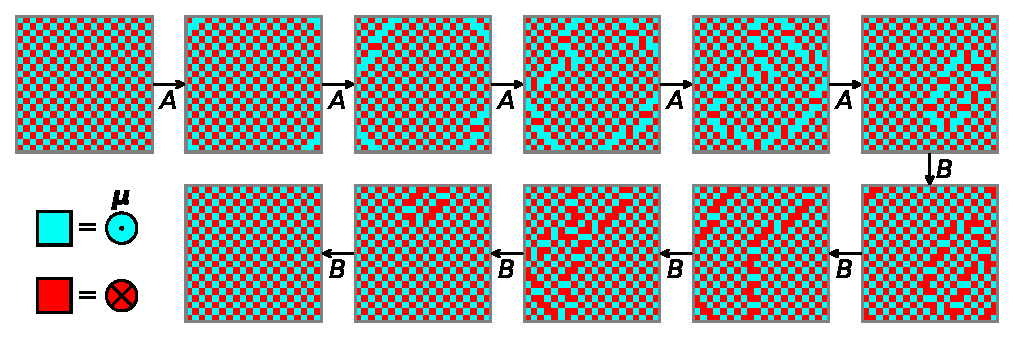
\includegraphics[width=\linewidth]{3_RC_OOP/Nonvolatile/Clocking_clearly_moments.pdf}
	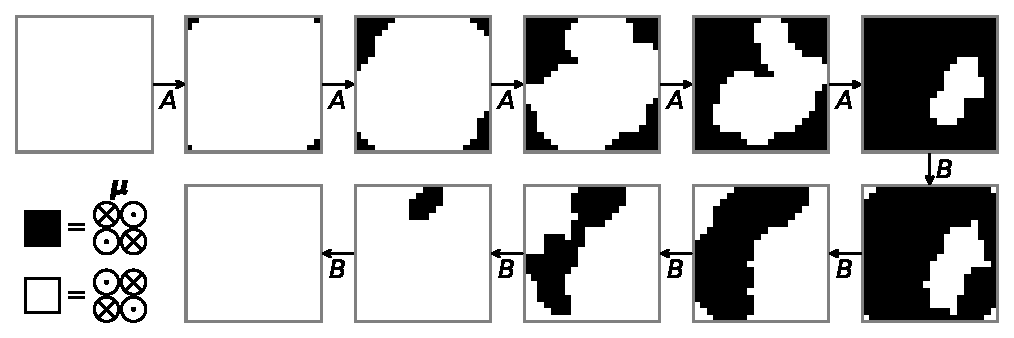
\includegraphics[width=\linewidth]{3_RC_OOP/Nonvolatile/Clocking_clearly_domains.pdf}
}{
	\label{fig:3:Clocking_clearly_domains}
	Evolution of a $20 \times 20$ OOP square-lattice ASI when using the two-step AFM clocking scheme (for five cycles $A$ and five opposite cycles $B$).
	The finite size of magnets was accounted for with $D_\mathrm{NM} = \SI{170}{\nano\metre}$ and $S_\mathrm{ASI} = \SI{200}{\nano\metre}$.
	System parameters were chosen to get $\EMC = 25 \kBT$ and $\EEA = 100 \kBT$, with $\sigma(\EEA) = \SI{5}{\percent}$.
	All magnets are initially magnetized in one of the antiferromagnetic ground states (black). The magnetic field used in the clocking cycles has a magnitude $B_\mathrm{ext} = \qty{48}{\milli\tesla}$, and each step is applied for \qty{0.5}{\second}.
}

Besides showing the magnetisation state of each magnet, \cref{fig:3:Clocking_clearly_domains} also shows the evolution of the spatial distribution of the two domain types.
The domain representation is more meaningful in this context, because the clocking scheme was designed to act on domains, promoting domains of one type during each cycle.
Therefore, only the domain representation will be used from here on.
\subsubsection{Input encoding} % Binary vs. byte etc. Sigmoid thingy?
% TODO: filter the simulations/sweeps that I performed and organise them below, have a look at what parameters were changed (E_B_std, binary/byte, endianness...)
